\chapter{Synthetic Nervous System Simulation}\label{ch:sns}
\graphicspath{{figs/60-sns/}{figs/60-sns/AnimatLab_reference/}}

The actuator and torque models of Chapters~\ref{ch:muscles} and~\ref{ch:torque} describe the robot's mechanics. Studying their interaction with neural control also requires a simulation that connects the mechanical model to a synthetic nervous system (SNS). I first attempted this integration in AnimatLab by combining a published walker with a spinal controller. The model produced stepping-like motion in air, but hand tuning did not produce walking. This chapter explains how that attempt motivated the development of software tools for assembling, testing, and comparing neuromechanical models.

\section{The AnimatLab Bipedal Walker}\label{sec:prior_walker}

For a course project in ME 610: Neuromechanical Modeling, Morrow and I combined the bipedal mechanics of \citet{li_bipedal_2017} with the two-level central pattern generator (CPG) of \citet{deng_neuromechanical_2019} in AnimatLab \citep{cofer_animatlab_2010}. The mechanical model had a pelvis and bilateral thigh, shank, foot, and toe segments, with sagittal-plane joints and antagonist Hill-type muscles at the hip, knee, and ankle. I added a passive toe joint. The initial controller used one rhythm generator (RG) to control both sides, with separate pattern-formation (PF) groups for each leg: one for the hip and one for the knee and ankle. The shared RG layer contained four neurons. We added afferent feedback at the motoneuron (MN) level. Figure~\ref{fig:animatlab_model_architecture} shows the model and controller organization.

I adjusted applied currents, synaptic weights, and muscle parameters by hand. The suspended model developed alternating muscle activity and stepping-like motion, presented at the 2021 NIH BRAIN Initiative Investigators Meeting \citep{bolenTorqueValuesArtificialKnee2021June15-17}. It did not achieve weight-bearing walking. The later bilateral-RG extension was a separate development; the suspended result does not establish its weight-bearing performance.

I subsequently expanded the neural model into left- and right-side circuits with interconnected rhythm generators (RGs). I constructed the right-side subsystems from the left-side organization and linked the two RGs through commissural pathways. This later model is referred to as the Walker Two-Layer (W2L) model. Further circuit schematics and implementation records are provided in Appendix~\ref{app:simulation_verification}.

The AnimatLab result established that the combined model could produce stepping-like motion under suspension, but it did not establish weight-bearing walking. It also left unanswered how the controller would behave with the human musculotendon mechanics or BPA routing used elsewhere in this project. Investigating those questions required a way to connect the circuit to each mechanical model, inspect its signals, and test the connections before interpreting whole-model behavior.

\begin{figure}[p]
\centering
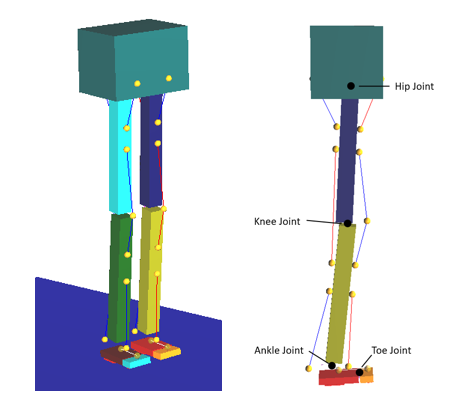
\includegraphics[width=0.64\textwidth,height=0.30\textheight,keepaspectratio]{OurWalker.png}
\par\medskip
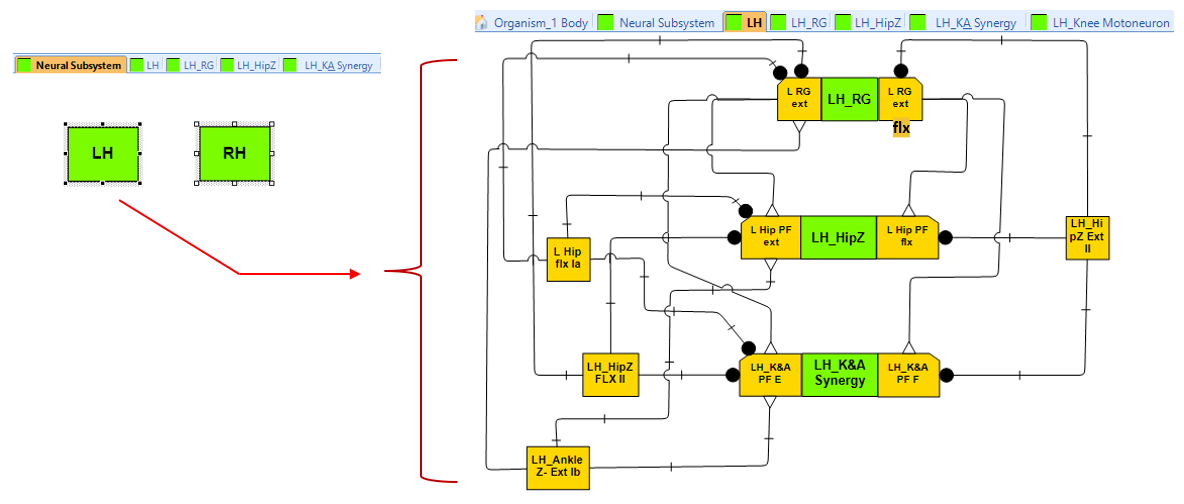
\includegraphics[width=\textwidth,height=0.31\textheight,keepaspectratio]{2layerImprove.png}
\caption[AnimatLab walker and controller hierarchy]{AnimatLab walker (top) and bilateral controller hierarchy (bottom). The model combines the Li walker mechanics and Deng CPG organization. These diagrams show construction; the suspended stepping result is described in the text.}
\label{fig:animatlab_model_architecture}
\end{figure}

\section{Knowledge Gaps and the New Tools}\label{sec:sns_gaps}

The suspended walker raised a question that its observed motion could not answer: which parts of the neural controller, sensory feedback, and mechanical model were responsible for the behavior? Changing several of them together could produce movement without showing why it occurred. Before using the simulation to study control of the robot, I needed to check the translated circuits and their mechanical connections separately, then examine the coupled model with controlled changes to its inputs or mechanics.

One gap concerned the mechanical model. The Li walker used simplified biological muscles, whereas this project also required a human musculoskeletal reference and a robot model with BPA routing and force production. A controller that produced motion in one of these models could not be assumed to work in the others. The OpenSim-to-MuJoCo conversion and BPA-force calculation made those comparisons possible. Their contribution was an inspectable connection between neural output, actuator force, and sensory return. Geometry and force-direction checks establish parts of that connection; they do not establish equivalent locomotion across the models.

A second gap concerned the controller itself. Transferring a circuit required preserving its connectivity, synaptic strengths, neuron dynamics, and sensory inputs. Agreement in burst timing could otherwise conceal a changed mechanism, such as a rhythm imposed by alternating contact inputs. Matched circuit tests therefore distinguish intrinsic rhythmic activity from sensory-driven alternation. Coupled perturbation tests then ask whether a controller continues to produce supported progression when the mechanics change while its conductances remain fixed.

A third gap was practical: the mechanical and neural models used different construction environments. Scripted MuJoCo and SNS-Toolbox models supported automated evaluations, while the MATLAB mechanical models and CAD-derived mechanisms needed a graphical neural interface. The SNS-Simscape library supplied editable neural and sensory blocks for that workflow. Its verification must address both circuit behavior and exchange of forces and measurements with a mechanical model. Importing a mechanism alone answers neither question. The following sections describe the tools and the tests that establish their present scope.

Existing software supplied separate parts of the solution. OpenSim supplied musculoskeletal geometry, MyoConverter translated it to MuJoCo, and SNS-Toolbox supplied neuron and synapse models \citep{delp_opensim_2007, caggiano_myosuite_2022, todorov_mujoco_2012, nourse_sns_2023}. The MuJoCo version used here supports scripted simulation and parameter searches but uses rigid tendons; its Python interface does not provide the block-based circuit assembly needed for this workflow. Simulink supplies that graphical construction, while Simscape Multibody imports mechanical geometry, including SolidWorks-derived mechanisms. AnimatLab retains the reference controllers but is unsupported, relies on an older physics engine, and ran these simulations slowly. The tools connect these complementary environments and use matched tests to check what transfers between them.

\section{Software Tools}\label{sec:preliminary_sim_methods}

The tools connect musculoskeletal geometry, actuator forces, and neural circuits. Figure~\ref{fig:pipeline} shows these connections and their relationship to the proposed hardware system.

\subsection{Model Conversion and Actuator Coupling}\label{sec:sns_existing_tools}

My first conversion attempt used the robot model, which combined BPA routing on the Gait2392 skeleton with unchanged human muscle parameters. MyoConverter's muscle-equilibrium checks rejected infeasible combinations of routed length and muscle parameters. I therefore separated conversion of the human reference from reconstruction of the robot routing. This distinction matters because an error caused by an artificial-actuator route should not be interpreted as a property of the original human model.

The human-model conversion also required specific repairs. Three small hip rotators per side, the quadratus femoris, gemelli, and piriformis, were disabled at model load. The converted model retains 92 actuator entries, but these six contribute no force. The model retains the OpenSim and International Society of Biomechanics coordinate convention; frame transformations and individual-actuator tests check that joint motion and torque directions have the intended signs.

The source represents patella motion through muscle insertion locations that vary with knee angle. In the converted model, limits on the joints representing these moving path points conflicted with their coupling constraints. Removing those conflicting limits allowed the coupled path points to follow their prescribed trajectories. The rectus femoris path also required a patella-tracking via point to restore its knee-extension action. Explicit collision pairs introduced unwanted contacts, so contact was restricted to the foot--ground pairs. Passive joint torques supplied joint-stop behavior absent from the conversion. These repairs explain why conversion needed checks beyond successful loading: a model could load while producing an incorrect torque direction or unintended contact force.

Comparisons with the OpenSim attachment paths and single-actuator tests checked the transferred geometry and force directions. They do not establish that every muscle reproduces the source force throughout its range or that the controller produces walking. The neural and mechanical models exchange signals at a \qty{2}{\milli\second} solver time step.

For the BPA-routed robot model, an actuator-force calculation connects the neural and mechanical simulations. It takes the simulated muscle length and pressure as inputs and evaluates the quasi-static force model from Chapter~\ref{ch:muscles}; the resulting force acts along the simulated actuator path. This calculation does not include valve or pressure dynamics. Length, velocity, force, and foot-contact signals return to the controller through sensory channels. The correction terms of Chapter~\ref{ch:torque} do not by themselves establish that transferred routing and compliance are correct in a dynamic model; those properties require separate checks.

\subsection{Graphical Circuit Construction}\label{sec:sns_new_tools}

The SNS-Simscape library implements neuron, synapse, afferent-encoder, activation, and muscle-force elements as editable Simulink blocks. The library retains the conductance-based neuron and synapse formulation supplied by SNS-Toolbox; it does not introduce a new neuron model. Verification uses selected circuits under matched inputs. Figure~\ref{fig:simulink_sns_implementation} shows the core blocks and graded-neuron signal flow.

Transcribing the source circuits also required distinguishing synapse-type parameters from per-instance editor fields. The Deng AnimatLab project contains 90 neurons, 196 synapses, and 58 named synapse types. Many instance fields retain a common editor default, while the named types specify different pathway conductances. The extraction records both fields so that a uniform default does not replace the source's pathway-specific strengths. A matching neuron count alone would not detect that error.

OpenSim-derived and SolidWorks-derived mechanisms were imported into Simscape Multibody. These mechanical imports are separate from the standalone reflex demonstrations.

\begin{figure}[htbp]
\centering
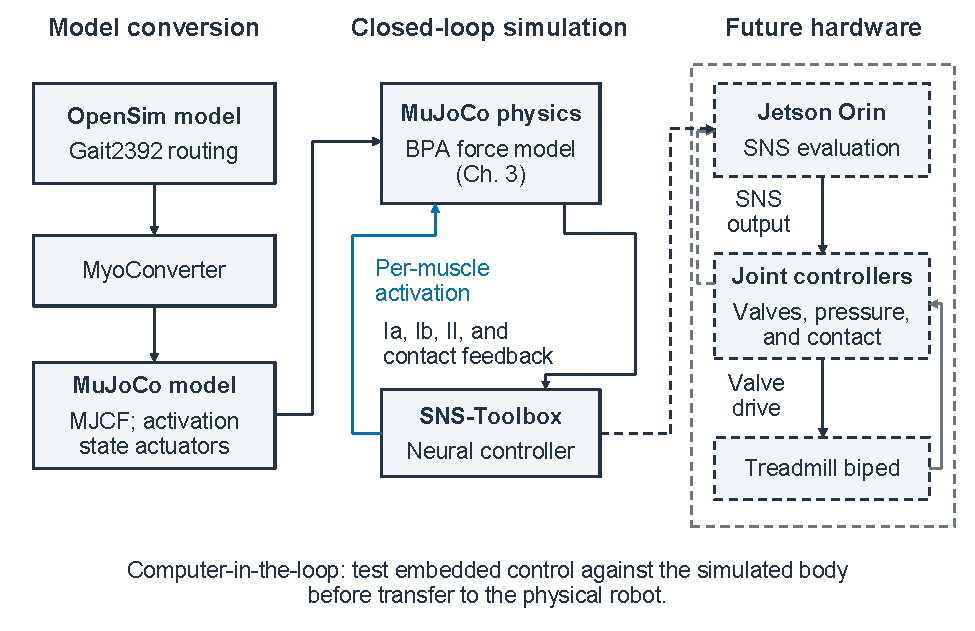
\includegraphics[width=\textwidth]{pipeline.pdf}
\caption[Simulation-to-robot pipeline]{Model conversion, closed-loop simulation, and proposed hardware deployment. Solid simulation interfaces connect neural activation to BPA force and return afferent signals. The embedded valve-control and network-evaluation system is future work (Chapter~\ref{ch:futurework}).}
\label{fig:pipeline}
\end{figure}

\begin{figure}[p]
\centering
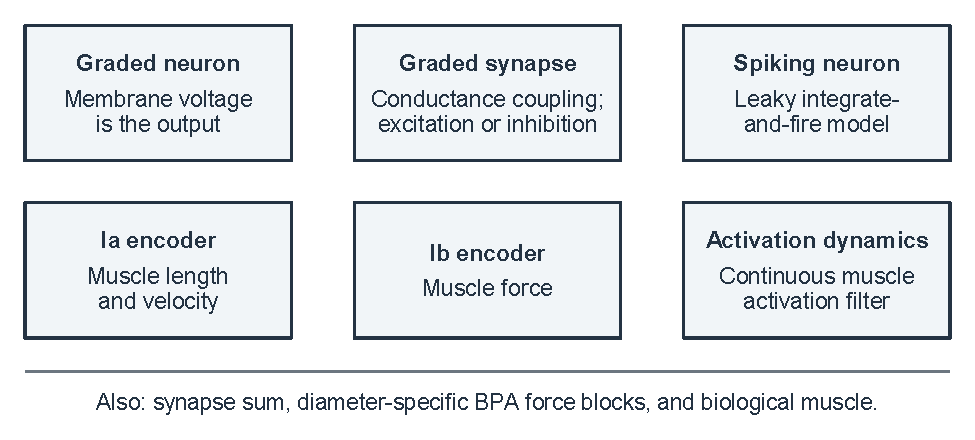
\includegraphics[width=0.94\textwidth,height=0.42\textheight,keepaspectratio]{sns_library_overview.pdf}
\par\medskip
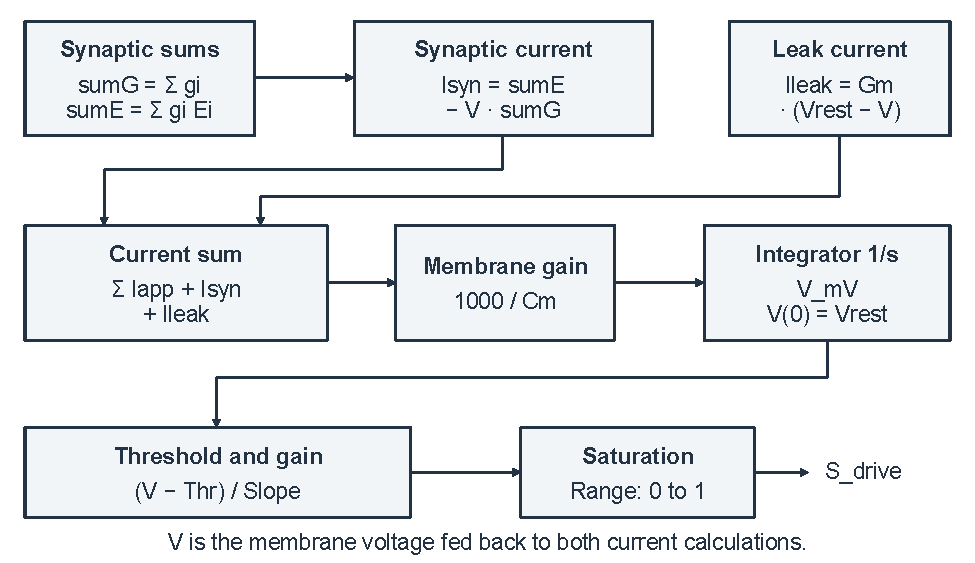
\includegraphics[width=0.94\textwidth]{simulink_neuron_detail.pdf}
\caption[Simulink SNS library blocks and neuron implementation]{Core SNS-Simscape blocks (top) and graded-neuron implementation (bottom). Summed currents drive membrane integration; threshold, inverse-slope gain, and saturation bound the output. Voltage feeds both current calculations. The generic BPA demonstration remains provisional.}
\label{fig:simulink_sns_implementation}
\end{figure}

\section{Verification of the Implemented Interfaces}\label{sec:preliminary_sim_results}

The tests address three distinct questions: whether a circuit produces its expected response, whether implementations agree under matched inputs, and whether the neural and mechanical models exchange signals in a closed loop.  The larger evaluation sets and their limitations are collected in Appendix~\ref{app:simulation_verification}; neuron equations and calibration details remain in Appendix~\ref{app:neuron_equations}.

\subsection{Reflex Response}\label{sec:sns_simulink_demos}

The library assembles Ia stretch excitation, reciprocal inhibition, and Ib autogenic inhibition in a reduced-order antagonist knee model (Figure~\ref{fig:simulink_reflex_topology}). A second demonstration tests the stretch reflex in an arm holding a beverage container as it is loaded. With the reflex enabled, arm sag was \ang{2.00}, compared with \ang{7.85} when it was disabled. The comparison checks the implemented feedback response; experimental calibration of the mechanical parameters remains necessary.

\begin{figure}[p]
\centering
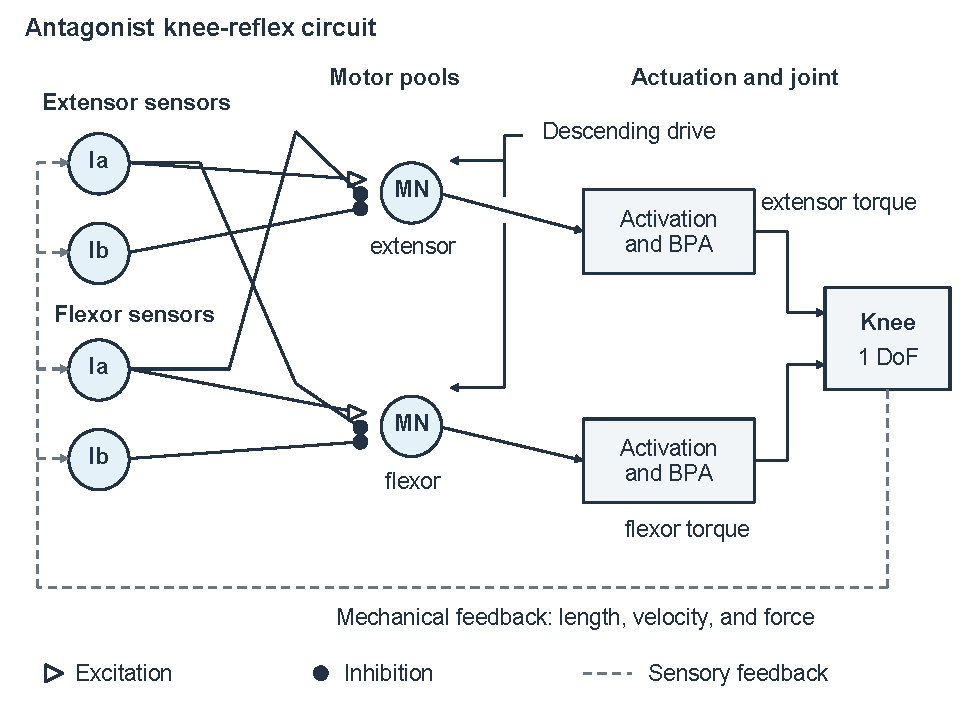
\includegraphics[width=\textwidth]{KneeReflex_circuit.pdf}
\caption[Reduced-order knee-reflex circuit topology]{Reduced-order antagonist knee-reflex circuit. Triangles mark excitation, and filled circles mark inhibition. Ia input excites the homonymous motor pool and inhibits its antagonist; Ib input inhibits the homonymous pool. Motor output drives activation and BPA-force blocks. Mechanical parameters and the generic BPA block remain provisional.}
\label{fig:simulink_reflex_topology}
\end{figure}

\subsection{Matched Neural Implementations}\label{sec:crossengine_results}

The contact-driven W2L rhythm core was implemented in NumPy and native Simulink blocks from a common connectivity specification. Both implementations received the same input protocol. Burst periods matched at \qty{1.000}{\second}, all ten expected bursts were reproduced, and voltage-trace correlation was at least 0.99996 (Figure~\ref{fig:w2l_crossengine}). The agreement is specific to this circuit and input protocol.

Removing the phasic heel-contact inputs caused the circuit to latch in both implementations. The alternating activity therefore depends on the specified sensory drive.

\begin{figure}[htbp]
\centering
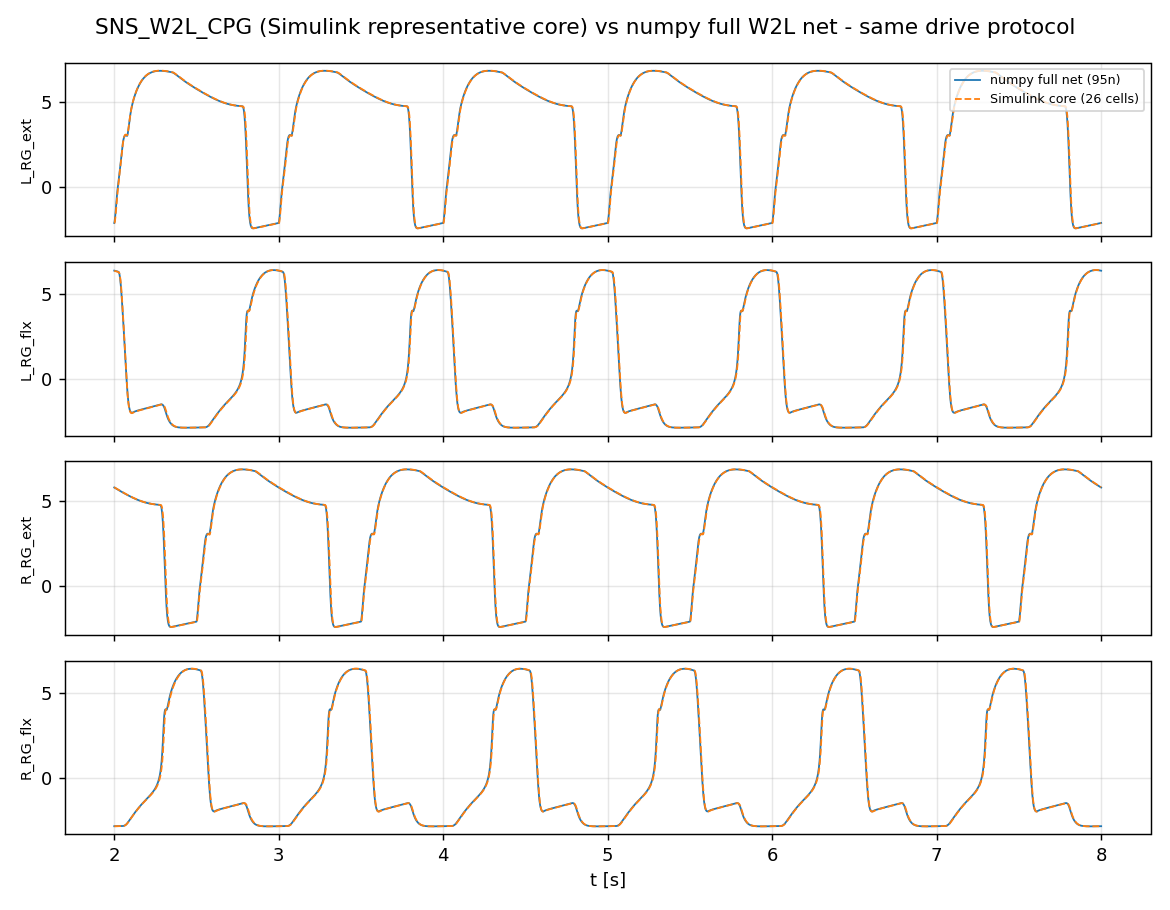
\includegraphics[width=\textwidth,height=0.55\textheight,keepaspectratio]{sns_w2l_traces.png}
\caption[W2L rhythm-core traces across engines]{W2L rhythm-generator voltages under matched inputs in NumPy and Simulink. Burst periods and counts agree; full-trace correlation is at least 0.99996. The residual \qty{2}{\milli\second} lag is one discrete solver time step. The test concerns the driven rhythm core, not walking mechanics.}
\label{fig:w2l_crossengine}
\end{figure}

A separate Simulink implementation of a Deng-derived RG/PF circuit, with a fixed sodium-inactivation time constant of \qty{350}{\milli\second}, produced ten bursts over \qty{20}{\second} following a single \qty{10}{\nano\ampere}, \qty{1}{\milli\second} pulse. Its period was \qty{1.938}{\second}, compared with approximately \qty{1.94}{\second} in the NumPy reference. This test demonstrates self-sustained activity after a brief input, unlike the contact-driven comparison above. It does not demonstrate pointwise voltage agreement: the logged maximum voltage differences were approximately \qty{63}{\milli\volt}.

Additional tests checked the graphical implementation at different scales. In the five-neuron SNS-Toolbox tutorial circuit, final membrane voltages agreed with the NumPy implementation to within \qty{1.1e-5}{\milli\volt}. The persistent-sodium tutorial pair reproduced its winner and loser steady states, but retained transient differences. For the 410-neuron export, the maximum difference across all final membrane voltages at \qty{0.3}{\second} was \qty{4.201e-6}{\milli\volt} with a \qty{2}{\milli\second} Euler time step. This short-window check tests translation of the network equations and wiring; it does not establish long-duration agreement or transfer of a tuned walking controller.

A Li-derived contact-driven circuit was also assembled with 58 neurons and 98 connections. This implementation substitutes graded stance cells with slow adaptation for the original spiking cells. Under scripted alternating heel inputs, it produced rhythmic activity with an inter-leg correlation of $-0.271$. It is an adaptation tested with imposed contacts, rather than a reproduction of the original circuit's closed-loop walking experiment.

\subsection{Closed-Loop Model Coupling}

The MuJoCo--Simulink bridge was tested against an independent Python integration using single-muscle activation, different control rates, and sensor readback. Readback was bit-exact over the scored window. The exported neural network also drove all 92 actuators during a \qty{5}{\second} open-loop run without afferent return. A separate reflex experiment exercised commands and sensory measurements through the interface. These tests establish selected force and signal paths across the interface, rather than a complete transferred locomotor controller.

The Simulink air-stepping demonstration connects eight BPA-force elements to two planar legs with a fixed pelvis and no ground contact. It establishes that neural commands can drive the actuator and joint calculations together. However, the approximately \qty{0.31}{\second} swing period differed substantially from the RG period of \qty{1.938}{\second}. The observed limb oscillation therefore does not establish that the mechanics follow the neural rhythm. Mechanical imports from OpenSim and SolidWorks remain another stage of integration; the standalone reflex and air-stepping demonstrations do not establish control of those imported mechanisms.

\subsection{Perturbation Robustness and Pathway Deletions}\label{sec:w2l_perturbation}

The coupled W2L evaluations address a different question from the circuit-translation tests: whether a fixed controller tolerates changes in the body. The recorded mass-change experiment held the controller settings fixed while scaling segment masses and inertias. Thigh or distal-leg properties were changed by $\pm10$ and $\pm20$ percent, and the whole leg by $\pm10$ percent. All ten recorded conditions met the campaign's supported-progression criterion during \qty{30}{\second} runs: finite simulation, no detected fall, at least six heel-contact cycles per leg, median inter-leg phase between 0.35 and 0.65, and forward displacement greater than \qty{0.05}{\metre}. The recorded forward displacements ranged from \qty{0.781}{\metre} to \qty{1.630}{\metre} over the scored windows.

These results concern the W2L mechanical model with a retained virtual harness, not the BPA-routed Gait2392 robot model. The harness supplied vertical feedback and constrained lateral motion, roll, and yaw. Its nominal weight-support setting was \qty{25}{\percent}; the realized vertical force also depended on the height-control terms. Thus the test demonstrates tolerance to the specified mechanical changes within the supported simulation, rather than unsupported balance or a constant \qty{25}{\percent} unloading force.

Separate searches reduced the nominal weight-support setting from 70 to 10 percent, with controller parameters allowed to change between settings. Each selected configuration passed a fresh-process \qty{30}{\second} evaluation. This is evidence that supported progression could be recovered at each tested setting; it is not a demonstration that one frozen controller tolerated the entire reduction. The local conductance-perturbation tests remained less robust: the selected configurations at nominal 25 and 10 percent support passed 9 and 7 of 12 probes, respectively, and both were recorded as failures of their acceptance criterion. Tolerance to segment-mass changes therefore should not be generalized to tolerance to arbitrary controller changes.

The parameter-loading implementation limits interpretation of these searches. Of the 61 conductance and encoding fields saved in the selected configuration, 55 individual pathway fields are excluded by the evaluator's accepted-key filter. The runner also does not forward those individual fields to the circuit builder. Consequently, the stored outcomes cannot establish that all saved conductances were optimized or applied. A replay that records the effective compiled conductances is needed to reconcile the selected configuration with the controller actually evaluated.

Exploratory network-deletion tests recorded 13 left-heel cycles after several nominal pathway removals, two after commissural removal, and zero after Ib-feedback removal. However, the corresponding summary counted the left heel again for its right-side column, and the runner does not forward several of the individual deletion settings. Unchanged output therefore cannot establish that a pathway was removed and compensated by other pathways. These records do not establish bilateral pathway necessity. Correctly applied deletions and independently scored bilateral contact and joint traces are needed before assigning that interpretation. Likewise, continued motion after a stimulus or push requires a defined recovery measure before it can establish recovery to the original gait.

A separate controller derived from \citet{dirusso_investigating_2023} was coupled to the Gait2392 human model. It uses per-muscle reflex parameters and a staged optimization procedure, with changes to the source model and optimization method. The recorded second-stage stability search completed 120 trials without a configuration passing its survival criterion. This is a negative result for that implementation and search, rather than a reproduction of the published walking result. It also shows why completing a connectome transcription or obtaining a fitted neural output cannot substitute for testing the coupled mechanics.

\section{Capabilities and Remaining Limits}\label{sec:sns_discussion}

The initial AnimatLab result showed suspended stepping-like motion but left its dependence on circuit organization, feedback, and mechanics unclear. The tools developed here make those dependencies testable in stages. Conversion repairs address whether forces act along the intended routes. Matched circuit tests address whether a translated implementation preserves selected neural responses. Coupled evaluations address how a controller behaves when its sensory input comes from the mechanical model. Keeping those questions separate prevents a successful component test from being treated as evidence for complete locomotion.

The new results strengthen specific parts of this chain. A brief-pulse test produced self-sustained neural bursts, short-window comparisons checked network translation, and the recorded mass-change tests retained supported progression in the W2L model. They also identify remaining problems: the Li transcription changes the neuron dynamics, the air-stepping mechanics do not yet follow the RG period, and parameter loading and deletion scoring require correction before the corresponding optimization and pathway claims can be accepted. None of these results establishes that the BPA-routed robot model reproduces the W2L result or that either model walks without a harness.

The resulting contribution is a set of neural, actuator, and mechanical interfaces with tests that distinguish implemented capabilities from unresolved model behavior. The next use of these tools is to compare controllers and feedback pathways under matched mechanical conditions, then evaluate whether the resulting behavior transfers to the robot. Chapter~\ref{ch:futurework} discusses hardware deployment and further extensions.
